%%%%%%%%%%%%%%%%%%%%%%%%%%%%%%%%%%%%%%%%%%%%%%%%%%%%%%%%%%%%%%%%%%%%%%%%%%%%%%%%%%%%%%%%%%%%%%%%%%%%%%%%%%%%%%%%%%%%%%%%%%%%%%%%%%%%%%%%%%%%%%%%%%%%%%%%%%%%%%%%%%%
% Written By Michael Brodskiy
% Class: Fundamentals of Linear Systems
% Professor: I. Salama
%%%%%%%%%%%%%%%%%%%%%%%%%%%%%%%%%%%%%%%%%%%%%%%%%%%%%%%%%%%%%%%%%%%%%%%%%%%%%%%%%%%%%%%%%%%%%%%%%%%%%%%%%%%%%%%%%%%%%%%%%%%%%%%%%%%%%%%%%%%%%%%%%%%%%%%%%%%%%%%%%%%

\include{Includes.tex}

\title{Homework 1}
\date{\today}
\author{Michael Brodskiy\\ \small Professor: I. Salama}

\begin{document}

\maketitle

\begin{enumerate}

  \item Express each of the following complex numbers in polar form and plot them

    \begin{enumerate}

      \item $8$

        $$r=\sqrt{8^2+0^2}=8$$
        $$\theta=0$$
        $$z(r,\theta)=r(\cos(\theta)+j\sin(\theta))$$
        $$z(8,0)=8(\cos(0)+j\sin(0))$$
        $$\therefore \text{ In polar: } \boxed{z=8}$$

        \begin{figure}[H]
          \centering
          \include{Figures/Fig1a}
          \caption{$z=8$ Plotted on the Imaginary Plane}
          \label{fig:1}
        \end{figure}

      \item $-5$

        $$r=\sqrt{(-5)^2+0^2}=5$$
        $$\theta=\pi$$
        $$z(r,\theta)=r(\cos(\theta)+j\sin(\theta))$$
        $$z(5,\pi)=5(\cos(\pi)+j\sin(\pi))$$
        $$\therefore \text{ In polar: } \boxed{z=-5=5e^{\pi j}}$$

        \begin{figure}[H]
          \centering
          \tikzset{every picture/.style={line width=0.75pt}} %set default line width to 0.75pt        

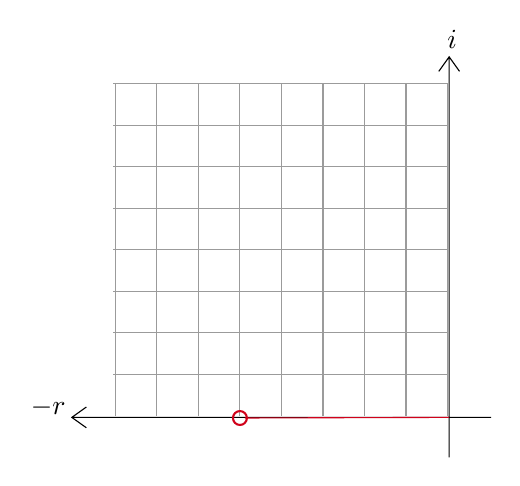
\begin{tikzpicture}[x=0.75pt,y=0.75pt,yscale=-1,xscale=1]
%uncomment if require: \path (0,300); %set diagram left start at 0, and has height of 300

%Shape: Axis 2D [id:dp5907524483347102] 
\draw  (469,209.7) -- (267,209.7)(448.8,36) -- (448.8,229) (274,204.7) -- (267,209.7) -- (274,214.7) (453.8,43) -- (448.8,36) -- (443.8,43)  ;
%Shape: Grid [id:dp6199898397920625] 
\draw  [draw opacity=0] (448,49) -- (287,49) -- (287,209) -- (448,209) -- cycle ; \draw  [color={rgb, 255:red, 155; green, 155; blue, 155 }  ,draw opacity=1 ] (448,49) -- (448,209)(428,49) -- (428,209)(408,49) -- (408,209)(388,49) -- (388,209)(368,49) -- (368,209)(348,49) -- (348,209)(328,49) -- (328,209)(308,49) -- (308,209)(288,49) -- (288,209) ; \draw  [color={rgb, 255:red, 155; green, 155; blue, 155 }  ,draw opacity=1 ] (448,49) -- (287,49)(448,69) -- (287,69)(448,89) -- (287,89)(448,109) -- (287,109)(448,129) -- (287,129)(448,149) -- (287,149)(448,169) -- (287,169)(448,189) -- (287,189) ; \draw  [color={rgb, 255:red, 155; green, 155; blue, 155 }  ,draw opacity=1 ]  ;
%Straight Lines [id:da9323494469903814] 
\draw [color={rgb, 255:red, 208; green, 2; blue, 27 }  ,draw opacity=1 ]   (448.8,209.7) -- (350.35,209.99) ;
\draw [shift={(348,210)}, rotate = 179.83] [color={rgb, 255:red, 208; green, 2; blue, 27 }  ,draw opacity=1 ][line width=0.75]      (0, 0) circle [x radius= 3.35, y radius= 3.35]   ;

% Text Node
\draw (450.23,33) node [anchor=south] [inner sep=0.75pt]    {$i$};
% Text Node
\draw (246,199.4) node [anchor=north west][inner sep=0.75pt]    {$-r$};

\end{tikzpicture}

          \caption{$z=-5$ Plotted on the Imaginary Plane}
          \label{fig:2}
        \end{figure}

      \item $2j$

        $$r=\sqrt{0^2+(2)^2}=2$$
        $$\theta=\frac{\pi}{2}$$
        $$z(r,\theta)=r(\cos(\theta)+j\sin(\theta))$$
        $$z(2,.5\pi)=2j$$
        $$\therefore \text{ In polar: } \boxed{z=2j=2e^{.5\pi j}}$$

        \begin{figure}[H]
          \centering
          \tikzset{every picture/.style={line width=0.75pt}} %set default line width to 0.75pt        

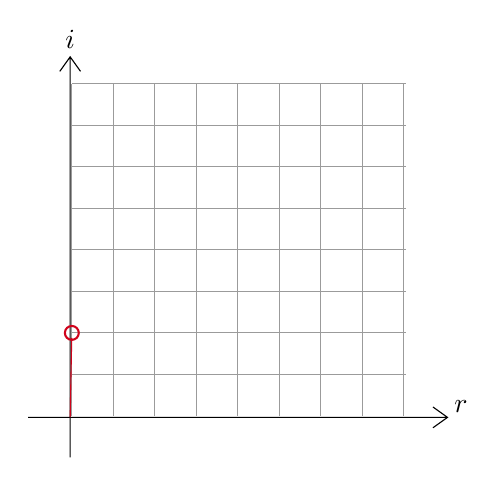
\begin{tikzpicture}[x=0.75pt,y=0.75pt,yscale=-1,xscale=1]
%uncomment if require: \path (0,300); %set diagram left start at 0, and has height of 300

%Shape: Axis 2D [id:dp5907524483347102] 
\draw  (267,209.7) -- (469,209.7)(287.2,36) -- (287.2,229) (462,204.7) -- (469,209.7) -- (462,214.7) (282.2,43) -- (287.2,36) -- (292.2,43)  ;
%Shape: Grid [id:dp6199898397920625] 
\draw  [draw opacity=0] (288,49) -- (449,49) -- (449,209) -- (288,209) -- cycle ; \draw  [color={rgb, 255:red, 155; green, 155; blue, 155 }  ,draw opacity=1 ] (288,49) -- (288,209)(308,49) -- (308,209)(328,49) -- (328,209)(348,49) -- (348,209)(368,49) -- (368,209)(388,49) -- (388,209)(408,49) -- (408,209)(428,49) -- (428,209)(448,49) -- (448,209) ; \draw  [color={rgb, 255:red, 155; green, 155; blue, 155 }  ,draw opacity=1 ] (288,49) -- (449,49)(288,69) -- (449,69)(288,89) -- (449,89)(288,109) -- (449,109)(288,129) -- (449,129)(288,149) -- (449,149)(288,169) -- (449,169)(288,189) -- (449,189) ; \draw  [color={rgb, 255:red, 155; green, 155; blue, 155 }  ,draw opacity=1 ]  ;
%Straight Lines [id:da9323494469903814] 
\draw [color={rgb, 255:red, 208; green, 2; blue, 27 }  ,draw opacity=1 ]   (287.2,209.7) -- (287.95,171.35) ;
\draw [shift={(288,169)}, rotate = 271.13] [color={rgb, 255:red, 208; green, 2; blue, 27 }  ,draw opacity=1 ][line width=0.75]      (0, 0) circle [x radius= 3.35, y radius= 3.35]   ;

% Text Node
\draw (287.23,33) node [anchor=south] [inner sep=0.75pt]    {$i$};
% Text Node
\draw (471,200.4) node [anchor=north west][inner sep=0.75pt]    {$r$};

\end{tikzpicture}

          \caption{$z=2j$ Plotted on the Imaginary Plane}
          \label{fig:3}
        \end{figure}

      \item $\frac{1}{4}(1-j)^5$

        $$.25(1-j)^2(1-j)^3$$
        $$.25(-2j)(1-j)(1-j)^2$$
        $$.25(-2-2j)(-2j)$$
        $$z=j-1$$
        $$r=\sqrt{1^2+(-1)^2}=\sqrt{2}$$
        $$\theta=\frac{3\pi}{4}$$
        $$z(r,\theta)=r(\cos(\theta)+j\sin(\theta))$$
        $$z(\sqrt{2},.75\pi)=j-1$$
        $$\therefore \text{ In polar: } \boxed{z=j-1=\sqrt{2}e^{.75\pi j}}$$

        \begin{figure}[H]
          \centering
          \include{Figures/Fig1d}
          \caption{$z=\frac{1}{4}(1-j)^5$ Plotted on the Imaginary Axis}
          \label{fig:4}
        \end{figure}

      \item $\frac{(1+j)}{j}e^{\frac{j\pi}{3}}$

        $$\frac{(1+j)}{j}\cdot\frac{-j}{-j}=1-j$$
        $$\tan\left( \frac{\pi}{3} \right)=\frac{b}{a}$$
        $$\frac{b}{a}=\sqrt{3}$$
        $$b=a\sqrt{3}$$
        $$\sqrt{(a\sqrt{3})^2+a^2}=1$$
        $$4a^2=\pm1$$
        $$a=\frac{1}{2}$$
        $$b=\frac{\sqrt{3}}{2}$$
        $$\frac{1}{2}(1-j)(1+\sqrt{3}j)\to\frac{1}{2}((\sqrt{3}+1)+(\sqrt{3}-1)j)$$
        $$r=\frac{1}{2}\sqrt{(\sqrt{3}+1)^2+(\sqrt{3}-1)^2}=\sqrt{(4+2\sqrt{3})+(4-2\sqrt{3})}$$
        $$r=\sqrt{2}$$
        $$\theta=\tan^{-1}\left( \frac{\sqrt{3}-1}{\sqrt{3}+1} \right)=.26179$$
        $$z(r,\theta)=r(\cos(\theta)+j\sin(\theta))$$
        $$z(\sqrt{2},.26179)=\frac{1}{2}(\sqrt{3}+1)+(\sqrt{3}-1)j$$
        $$\therefore \text{ In polar: } \boxed{z=\frac{1}{2}(\sqrt{3}+1)+(\sqrt{3}-1)j=\sqrt{2}e^{.26179j}}$$

        \begin{figure}[H]
          \centering
          \include{Figures/Fig1e}
          \caption{$z=\frac{(1+j)}{j}e^{\frac{j\pi}{3}}$ Plotted on the Imaginary Axis}
          \label{fig:5}
        \end{figure}

      \item $(\sqrt{3}-j^5)(1+j)$

        $$j^5=j\to (\sqrt{3}-j)(1+j)=(\sqrt{3}+(\sqrt{3}-1)j+1)$$
        $$(\sqrt{3}+1)+(\sqrt{3}-1)j$$
        $$r=\sqrt{(\sqrt{3}+1)^2+(\sqrt{3}-1)^2}=\sqrt{(4+2\sqrt{3})+(4-2\sqrt{3})}$$
        $$r=\sqrt{8}=2\sqrt{2}$$
        $$\theta=\tan^{-1}\left( \frac{\sqrt{3}-1}{\sqrt{3}+1} \right)=.26179$$
        $$z(r,\theta)=r(\cos(\theta)+j\sin(\theta))$$
        $$z(2\sqrt{2},.26179)=(\sqrt{3}+1)+(\sqrt{3}-1)j$$
        $$\therefore \text{ In polar: } \boxed{z=(\sqrt{3}+1)+(\sqrt{3}-1)j=2\sqrt{2}e^{.26179j}}$$

        \begin{figure}[H]
          \centering
          \include{Figures/Fig1f}
          \caption{$z=(\sqrt{3}-j^5)(1+j)$ Plotted on the Imaginary Axis}
          \label{fig:6}
        \end{figure}

      \item $\frac{2(\sqrt{3}-j)}{1+j\sqrt{3}}$

        $$\frac{2\sqrt{3}-2j}{1+j\sqrt{3}}\cdot\frac{1-j\sqrt{3}}{1-j\sqrt{3}}=-2j$$
        $$r=\sqrt{0^2+(-2)^2}=2$$
        $$\theta=\frac{3\pi}{2}$$
        $$z(r,\theta)=r(\cos(\theta)+j\sin(\theta))$$
        $$z(2,1.5\pi)=-2j$$
        $$\therefore \text{ In polar: } \boxed{z=-2j=2e^{1.5\pi j}}$$

        \begin{figure}[H]
          \centering
          \tikzset{every picture/.style={line width=0.75pt}} %set default line width to 0.75pt        

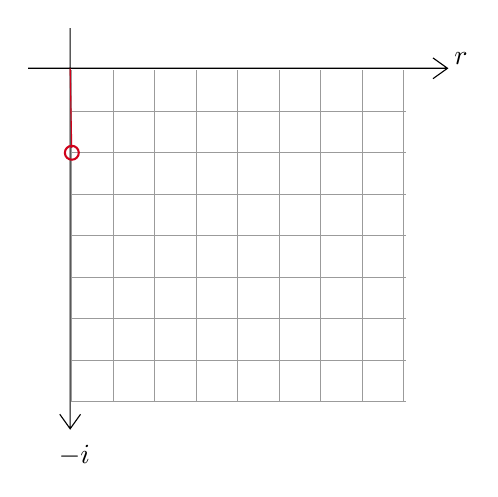
\begin{tikzpicture}[x=0.75pt,y=0.75pt,yscale=-1,xscale=1]
%uncomment if require: \path (0,300); %set diagram left start at 0, and has height of 300

%Shape: Axis 2D [id:dp5907524483347102] 
\draw  (267,55.3) -- (469,55.3)(287.2,229) -- (287.2,36) (462,60.3) -- (469,55.3) -- (462,50.3) (282.2,222) -- (287.2,229) -- (292.2,222)  ;
%Shape: Grid [id:dp6199898397920625] 
\draw  [draw opacity=0] (288,216) -- (449,216) -- (449,56) -- (288,56) -- cycle ; \draw  [color={rgb, 255:red, 155; green, 155; blue, 155 }  ,draw opacity=1 ] (288,216) -- (288,56)(308,216) -- (308,56)(328,216) -- (328,56)(348,216) -- (348,56)(368,216) -- (368,56)(388,216) -- (388,56)(408,216) -- (408,56)(428,216) -- (428,56)(448,216) -- (448,56) ; \draw  [color={rgb, 255:red, 155; green, 155; blue, 155 }  ,draw opacity=1 ] (288,216) -- (449,216)(288,196) -- (449,196)(288,176) -- (449,176)(288,156) -- (449,156)(288,136) -- (449,136)(288,116) -- (449,116)(288,96) -- (449,96)(288,76) -- (449,76) ; \draw  [color={rgb, 255:red, 155; green, 155; blue, 155 }  ,draw opacity=1 ]  ;
%Straight Lines [id:da9323494469903814] 
\draw [color={rgb, 255:red, 208; green, 2; blue, 27 }  ,draw opacity=1 ]   (287.2,55.3) -- (287.95,93.65) ;
\draw [shift={(288,96)}, rotate = 88.87] [color={rgb, 255:red, 208; green, 2; blue, 27 }  ,draw opacity=1 ][line width=0.75]      (0, 0) circle [x radius= 3.35, y radius= 3.35]   ;

% Text Node
\draw (289.23,248) node [anchor=south] [inner sep=0.75pt]    {$-i$};
% Text Node
\draw (471,46.4) node [anchor=north west][inner sep=0.75pt]    {$r$};

\end{tikzpicture}

          \caption{$z=\frac{2(\sqrt{3}-j)}{1+j\sqrt{3}}$ Plotted on the Imaginary Axis}
          \label{fig:7}
        \end{figure}

    \end{enumerate}

  \item Determine the value of $E_{\infty}$ and $P_{\infty}$ for each of the following signals and indicate whether the signal is a power or energy signal or neither.

    \begin{enumerate}

      \item $x_1(t)=\left\{\begin{array}{l r} 5e^{j(4t+\pi/3)},\, & t\geq 2\\ 0,\, & \text{Otherwise}\end{array}$

          $$|x_1(t)|=\sqrt{\left( 5\cos\left( 4t+\frac{\pi}{3} \right) \right)^2+\left( 5\sin\left( 4t+\frac{\pi}{3} \right) \right)^2}$$
          $$|x_1(t)|=5\sqrt{2}$$

          $$E_{\infty}=\int_2^{\infty} 50\,dt$$
          $$E_{\infty}=\infty$$
          $$\therefore\text{ Energy is infinite}$$

          $$P_{\infty}=\lim_{T\to\infty}\frac{1}{T}\int_{-T/2}^{T/2}50\,dt$$
          $$P_{\infty}=50$$
          $$\therefore\text{ Power is finite}$$

          $$\boxed{\text{Therefore, this is a power signal}}$$

      \item $x_2(t)=\left\{\begin{array}{l r} 2+2\cos(t),\, & 0<t< 2\pi\\ 0,\, & \text{Otherwise}\end{array}$

          $$P_{\infty}=\lim_{T\to\infty}\frac{1}{2T}\int_{-T}^{T}(2+2\cos(t))^2\,dt$$
          $$P_{\infty}=6$$
          $$\therefore\text{ Power is finite}$$

          $$E_{\infty}=\lim_{T\to\infty}\int_{-T}^T(2+2\cos(t))^2\,dt$$
          $$E_{\infty}=\infty$$
          $$\therefore\text{ Energy is infinite}$$

          \begin{center}
            $$\boxed{\text{Since power is finite and energy is infinite, this is a power signal}}$$
          \end{center}

        \item $x_3[n]=\left\{\begin{array}{l r} (.5)^n,\, & n\geq0\\ 0,\, & \text{Otherwise}\end{array}$

            $$E_{\infty}=\lim_{N\to\infty}\sum_{n=0}^N \left( .25 \right)^n$$
            \begin{center}
              A geometric series must be finite:
            \end{center}
            $$E_{\infty}\approx \left( \frac{1}{1-.25} \right)\approx \frac{4}{3}$$

            $$P_{\infty}=\lim_{N\to\infty}\frac{4/3}{2N+1}\approx 0$$

            \begin{center}
              $\boxed{\text{As such, because energy is finite and average power is 0, this is an energy signal}}$
            \end{center}

    \end{enumerate}

  \item For the discrete time signal shown in Figure P1.3, sketch, and carefully label each of the following.

    \begin{enumerate}

      \item $x[n-4]$

        \begin{figure}[H]
          \centering
          \tikzset{every picture/.style={line width=0.75pt}} %set default line width to 0.75pt        

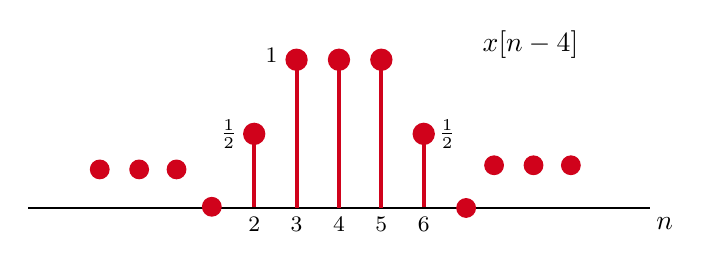
\begin{tikzpicture}[x=0.75pt,y=0.75pt,yscale=-1,xscale=1]
%uncomment if require: \path (0,364); %set diagram left start at 0, and has height of 364

%Straight Lines [id:da06072638558515686] 
\draw    (378.71,168) -- (79.29,168) ;
%Straight Lines [id:da5547538617459793] 
\draw [color={rgb, 255:red, 208; green, 2; blue, 27 }  ,draw opacity=1 ][fill={rgb, 255:red, 208; green, 2; blue, 27 }  ,fill opacity=1 ][line width=1.5]    (229,96.58) -- (229,168) ;
\draw [shift={(229,96.58)}, rotate = 90] [color={rgb, 255:red, 208; green, 2; blue, 27 }  ,draw opacity=1 ][fill={rgb, 255:red, 208; green, 2; blue, 27 }  ,fill opacity=1 ][line width=1.5]      (0, 0) circle [x radius= 4.36, y radius= 4.36]   ;
%Straight Lines [id:da08967735559368817] 
\draw [color={rgb, 255:red, 208; green, 2; blue, 27 }  ,draw opacity=1 ][fill={rgb, 255:red, 208; green, 2; blue, 27 }  ,fill opacity=1 ][line width=1.5]    (249.42,96.58) -- (249.42,168) ;
\draw [shift={(249.42,96.58)}, rotate = 90] [color={rgb, 255:red, 208; green, 2; blue, 27 }  ,draw opacity=1 ][fill={rgb, 255:red, 208; green, 2; blue, 27 }  ,fill opacity=1 ][line width=1.5]      (0, 0) circle [x radius= 4.36, y radius= 4.36]   ;
%Straight Lines [id:da11193473546126165] 
\draw [color={rgb, 255:red, 208; green, 2; blue, 27 }  ,draw opacity=1 ][fill={rgb, 255:red, 208; green, 2; blue, 27 }  ,fill opacity=1 ][line width=1.5]    (208.58,96.58) -- (208.58,168) ;
\draw [shift={(208.58,96.58)}, rotate = 90] [color={rgb, 255:red, 208; green, 2; blue, 27 }  ,draw opacity=1 ][fill={rgb, 255:red, 208; green, 2; blue, 27 }  ,fill opacity=1 ][line width=1.5]      (0, 0) circle [x radius= 4.36, y radius= 4.36]   ;
%Straight Lines [id:da8545689410720038] 
\draw [color={rgb, 255:red, 208; green, 2; blue, 27 }  ,draw opacity=1 ][fill={rgb, 255:red, 208; green, 2; blue, 27 }  ,fill opacity=1 ][line width=1.5]    (269.84,132.29) -- (269.84,167.71) ;
\draw [shift={(269.84,132.29)}, rotate = 90] [color={rgb, 255:red, 208; green, 2; blue, 27 }  ,draw opacity=1 ][fill={rgb, 255:red, 208; green, 2; blue, 27 }  ,fill opacity=1 ][line width=1.5]      (0, 0) circle [x radius= 4.36, y radius= 4.36]   ;
%Straight Lines [id:da9437858155461635] 
\draw [color={rgb, 255:red, 208; green, 2; blue, 27 }  ,draw opacity=1 ][fill={rgb, 255:red, 208; green, 2; blue, 27 }  ,fill opacity=1 ][line width=1.5]    (188.16,132.29) -- (188.16,167.71) ;
\draw [shift={(188.16,132.29)}, rotate = 90] [color={rgb, 255:red, 208; green, 2; blue, 27 }  ,draw opacity=1 ][fill={rgb, 255:red, 208; green, 2; blue, 27 }  ,fill opacity=1 ][line width=1.5]      (0, 0) circle [x radius= 4.36, y radius= 4.36]   ;
%Shape: Circle [id:dp8415745106048833] 
\draw  [color={rgb, 255:red, 208; green, 2; blue, 27 }  ,draw opacity=1 ][fill={rgb, 255:red, 208; green, 2; blue, 27 }  ,fill opacity=1 ] (163.24,167.42) .. controls (163.24,164.94) and (165.25,162.92) .. (167.74,162.92) .. controls (170.22,162.92) and (172.24,164.94) .. (172.24,167.42) .. controls (172.24,169.91) and (170.22,171.92) .. (167.74,171.92) .. controls (165.25,171.92) and (163.24,169.91) .. (163.24,167.42) -- cycle ;
%Shape: Circle [id:dp1924487381459985] 
\draw  [color={rgb, 255:red, 208; green, 2; blue, 27 }  ,draw opacity=1 ][fill={rgb, 255:red, 208; green, 2; blue, 27 }  ,fill opacity=1 ] (285.76,168) .. controls (285.76,165.51) and (287.78,163.5) .. (290.26,163.5) .. controls (292.75,163.5) and (294.76,165.51) .. (294.76,168) .. controls (294.76,170.49) and (292.75,172.5) .. (290.26,172.5) .. controls (287.78,172.5) and (285.76,170.49) .. (285.76,168) -- cycle ;
%Shape: Circle [id:dp9724739272897065] 
\draw  [color={rgb, 255:red, 208; green, 2; blue, 27 }  ,draw opacity=1 ][fill={rgb, 255:red, 208; green, 2; blue, 27 }  ,fill opacity=1 ] (146.24,149.42) .. controls (146.24,146.94) and (148.25,144.92) .. (150.74,144.92) .. controls (153.22,144.92) and (155.24,146.94) .. (155.24,149.42) .. controls (155.24,151.91) and (153.22,153.92) .. (150.74,153.92) .. controls (148.25,153.92) and (146.24,151.91) .. (146.24,149.42) -- cycle ;
%Shape: Circle [id:dp37116477968769124] 
\draw  [color={rgb, 255:red, 208; green, 2; blue, 27 }  ,draw opacity=1 ][fill={rgb, 255:red, 208; green, 2; blue, 27 }  ,fill opacity=1 ] (128.24,149.42) .. controls (128.24,146.94) and (130.25,144.92) .. (132.74,144.92) .. controls (135.22,144.92) and (137.24,146.94) .. (137.24,149.42) .. controls (137.24,151.91) and (135.22,153.92) .. (132.74,153.92) .. controls (130.25,153.92) and (128.24,151.91) .. (128.24,149.42) -- cycle ;
%Shape: Circle [id:dp0005769558109711692] 
\draw  [color={rgb, 255:red, 208; green, 2; blue, 27 }  ,draw opacity=1 ][fill={rgb, 255:red, 208; green, 2; blue, 27 }  ,fill opacity=1 ] (109.24,149.42) .. controls (109.24,146.94) and (111.25,144.92) .. (113.74,144.92) .. controls (116.22,144.92) and (118.24,146.94) .. (118.24,149.42) .. controls (118.24,151.91) and (116.22,153.92) .. (113.74,153.92) .. controls (111.25,153.92) and (109.24,151.91) .. (109.24,149.42) -- cycle ;
%Shape: Circle [id:dp5765900568262574] 
\draw  [color={rgb, 255:red, 208; green, 2; blue, 27 }  ,draw opacity=1 ][fill={rgb, 255:red, 208; green, 2; blue, 27 }  ,fill opacity=1 ] (336.24,147.42) .. controls (336.24,144.94) and (338.25,142.92) .. (340.74,142.92) .. controls (343.22,142.92) and (345.24,144.94) .. (345.24,147.42) .. controls (345.24,149.91) and (343.22,151.92) .. (340.74,151.92) .. controls (338.25,151.92) and (336.24,149.91) .. (336.24,147.42) -- cycle ;
%Shape: Circle [id:dp3702216225275915] 
\draw  [color={rgb, 255:red, 208; green, 2; blue, 27 }  ,draw opacity=1 ][fill={rgb, 255:red, 208; green, 2; blue, 27 }  ,fill opacity=1 ] (318.24,147.42) .. controls (318.24,144.94) and (320.25,142.92) .. (322.74,142.92) .. controls (325.22,142.92) and (327.24,144.94) .. (327.24,147.42) .. controls (327.24,149.91) and (325.22,151.92) .. (322.74,151.92) .. controls (320.25,151.92) and (318.24,149.91) .. (318.24,147.42) -- cycle ;
%Shape: Circle [id:dp5762492676349926] 
\draw  [color={rgb, 255:red, 208; green, 2; blue, 27 }  ,draw opacity=1 ][fill={rgb, 255:red, 208; green, 2; blue, 27 }  ,fill opacity=1 ] (299.24,147.42) .. controls (299.24,144.94) and (301.25,142.92) .. (303.74,142.92) .. controls (306.22,142.92) and (308.24,144.94) .. (308.24,147.42) .. controls (308.24,149.91) and (306.22,151.92) .. (303.74,151.92) .. controls (301.25,151.92) and (299.24,149.91) .. (299.24,147.42) -- cycle ;

% Text Node
\draw (380.71,171.4) node [anchor=north west][inner sep=0.75pt]    {$n$};
% Text Node
\draw (181.16,132.29) node [anchor=east] [inner sep=0.75pt]  [font=\footnotesize]  {$\frac{1}{2}$};
% Text Node
\draw (275.84,132.29) node [anchor=west] [inner sep=0.75pt]  [font=\footnotesize]  {$\frac{1}{2}$};
% Text Node
\draw (200.58,94.58) node [anchor=east] [inner sep=0.75pt]  [font=\footnotesize]  {$1$};
% Text Node
\draw (188.16,171.11) node [anchor=north] [inner sep=0.75pt]  [font=\footnotesize]  {$2$};
% Text Node
\draw (208.58,171.4) node [anchor=north] [inner sep=0.75pt]  [font=\footnotesize]  {$3$};
% Text Node
\draw (229,171.4) node [anchor=north] [inner sep=0.75pt]  [font=\footnotesize]  {$4$};
% Text Node
\draw (249.42,171.4) node [anchor=north] [inner sep=0.75pt]  [font=\footnotesize]  {$5$};
% Text Node
\draw (269.84,171.11) node [anchor=north] [inner sep=0.75pt]  [font=\footnotesize]  {$6$};
% Text Node
\draw (297,81.4) node [anchor=north west][inner sep=0.75pt]    {$x[ n-4]$};


\end{tikzpicture}

          \label{fig:8}
        \end{figure}

      \item $x[2n+2]$

        \begin{figure}[H]
          \centering
          \tikzset{every picture/.style={line width=0.75pt}} %set default line width to 0.75pt        

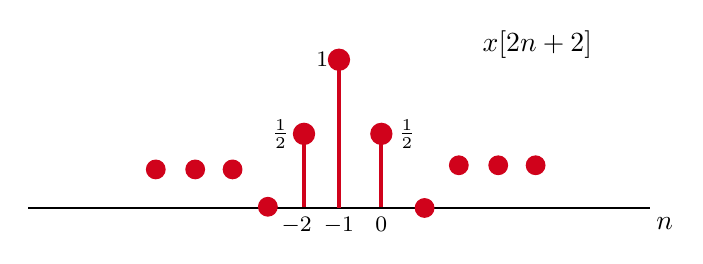
\begin{tikzpicture}[x=0.75pt,y=0.75pt,yscale=-1,xscale=1]
%uncomment if require: \path (0,364); %set diagram left start at 0, and has height of 364

%Straight Lines [id:da06072638558515686] 
\draw    (378.71,168) -- (79.29,168) ;
%Straight Lines [id:da5547538617459793] 
\draw [color={rgb, 255:red, 208; green, 2; blue, 27 }  ,draw opacity=1 ][fill={rgb, 255:red, 208; green, 2; blue, 27 }  ,fill opacity=1 ][line width=1.5]    (229,96.58) -- (229,168) ;
\draw [shift={(229,96.58)}, rotate = 90] [color={rgb, 255:red, 208; green, 2; blue, 27 }  ,draw opacity=1 ][fill={rgb, 255:red, 208; green, 2; blue, 27 }  ,fill opacity=1 ][line width=1.5]      (0, 0) circle [x radius= 4.36, y radius= 4.36]   ;
%Straight Lines [id:da8545689410720038] 
\draw [color={rgb, 255:red, 208; green, 2; blue, 27 }  ,draw opacity=1 ][fill={rgb, 255:red, 208; green, 2; blue, 27 }  ,fill opacity=1 ][line width=1.5]    (249.42,132.29) -- (249.42,167.71) ;
\draw [shift={(249.42,132.29)}, rotate = 90] [color={rgb, 255:red, 208; green, 2; blue, 27 }  ,draw opacity=1 ][fill={rgb, 255:red, 208; green, 2; blue, 27 }  ,fill opacity=1 ][line width=1.5]      (0, 0) circle [x radius= 4.36, y radius= 4.36]   ;
%Straight Lines [id:da9437858155461635] 
\draw [color={rgb, 255:red, 208; green, 2; blue, 27 }  ,draw opacity=1 ][fill={rgb, 255:red, 208; green, 2; blue, 27 }  ,fill opacity=1 ][line width=1.5]    (212.16,132.29) -- (212.16,167.71) ;
\draw [shift={(212.16,132.29)}, rotate = 90] [color={rgb, 255:red, 208; green, 2; blue, 27 }  ,draw opacity=1 ][fill={rgb, 255:red, 208; green, 2; blue, 27 }  ,fill opacity=1 ][line width=1.5]      (0, 0) circle [x radius= 4.36, y radius= 4.36]   ;
%Shape: Circle [id:dp8415745106048833] 
\draw  [color={rgb, 255:red, 208; green, 2; blue, 27 }  ,draw opacity=1 ][fill={rgb, 255:red, 208; green, 2; blue, 27 }  ,fill opacity=1 ] (190.24,167.42) .. controls (190.24,164.94) and (192.25,162.92) .. (194.74,162.92) .. controls (197.22,162.92) and (199.24,164.94) .. (199.24,167.42) .. controls (199.24,169.91) and (197.22,171.92) .. (194.74,171.92) .. controls (192.25,171.92) and (190.24,169.91) .. (190.24,167.42) -- cycle ;
%Shape: Circle [id:dp1924487381459985] 
\draw  [color={rgb, 255:red, 208; green, 2; blue, 27 }  ,draw opacity=1 ][fill={rgb, 255:red, 208; green, 2; blue, 27 }  ,fill opacity=1 ] (265.76,168) .. controls (265.76,165.51) and (267.78,163.5) .. (270.26,163.5) .. controls (272.75,163.5) and (274.76,165.51) .. (274.76,168) .. controls (274.76,170.49) and (272.75,172.5) .. (270.26,172.5) .. controls (267.78,172.5) and (265.76,170.49) .. (265.76,168) -- cycle ;
%Shape: Circle [id:dp9724739272897065] 
\draw  [color={rgb, 255:red, 208; green, 2; blue, 27 }  ,draw opacity=1 ][fill={rgb, 255:red, 208; green, 2; blue, 27 }  ,fill opacity=1 ] (173.24,149.42) .. controls (173.24,146.94) and (175.25,144.92) .. (177.74,144.92) .. controls (180.22,144.92) and (182.24,146.94) .. (182.24,149.42) .. controls (182.24,151.91) and (180.22,153.92) .. (177.74,153.92) .. controls (175.25,153.92) and (173.24,151.91) .. (173.24,149.42) -- cycle ;
%Shape: Circle [id:dp37116477968769124] 
\draw  [color={rgb, 255:red, 208; green, 2; blue, 27 }  ,draw opacity=1 ][fill={rgb, 255:red, 208; green, 2; blue, 27 }  ,fill opacity=1 ] (155.24,149.42) .. controls (155.24,146.94) and (157.25,144.92) .. (159.74,144.92) .. controls (162.22,144.92) and (164.24,146.94) .. (164.24,149.42) .. controls (164.24,151.91) and (162.22,153.92) .. (159.74,153.92) .. controls (157.25,153.92) and (155.24,151.91) .. (155.24,149.42) -- cycle ;
%Shape: Circle [id:dp0005769558109711692] 
\draw  [color={rgb, 255:red, 208; green, 2; blue, 27 }  ,draw opacity=1 ][fill={rgb, 255:red, 208; green, 2; blue, 27 }  ,fill opacity=1 ] (136.24,149.42) .. controls (136.24,146.94) and (138.25,144.92) .. (140.74,144.92) .. controls (143.22,144.92) and (145.24,146.94) .. (145.24,149.42) .. controls (145.24,151.91) and (143.22,153.92) .. (140.74,153.92) .. controls (138.25,153.92) and (136.24,151.91) .. (136.24,149.42) -- cycle ;
%Shape: Circle [id:dp5765900568262574] 
\draw  [color={rgb, 255:red, 208; green, 2; blue, 27 }  ,draw opacity=1 ][fill={rgb, 255:red, 208; green, 2; blue, 27 }  ,fill opacity=1 ] (319.24,147.42) .. controls (319.24,144.94) and (321.25,142.92) .. (323.74,142.92) .. controls (326.22,142.92) and (328.24,144.94) .. (328.24,147.42) .. controls (328.24,149.91) and (326.22,151.92) .. (323.74,151.92) .. controls (321.25,151.92) and (319.24,149.91) .. (319.24,147.42) -- cycle ;
%Shape: Circle [id:dp3702216225275915] 
\draw  [color={rgb, 255:red, 208; green, 2; blue, 27 }  ,draw opacity=1 ][fill={rgb, 255:red, 208; green, 2; blue, 27 }  ,fill opacity=1 ] (301.24,147.42) .. controls (301.24,144.94) and (303.25,142.92) .. (305.74,142.92) .. controls (308.22,142.92) and (310.24,144.94) .. (310.24,147.42) .. controls (310.24,149.91) and (308.22,151.92) .. (305.74,151.92) .. controls (303.25,151.92) and (301.24,149.91) .. (301.24,147.42) -- cycle ;
%Shape: Circle [id:dp5762492676349926] 
\draw  [color={rgb, 255:red, 208; green, 2; blue, 27 }  ,draw opacity=1 ][fill={rgb, 255:red, 208; green, 2; blue, 27 }  ,fill opacity=1 ] (282.24,147.42) .. controls (282.24,144.94) and (284.25,142.92) .. (286.74,142.92) .. controls (289.22,142.92) and (291.24,144.94) .. (291.24,147.42) .. controls (291.24,149.91) and (289.22,151.92) .. (286.74,151.92) .. controls (284.25,151.92) and (282.24,149.91) .. (282.24,147.42) -- cycle ;

% Text Node
\draw (380.71,171.4) node [anchor=north west][inner sep=0.75pt]    {$n$};
% Text Node
\draw (206.16,132.29) node [anchor=east] [inner sep=0.75pt]  [font=\footnotesize]  {$\frac{1}{2}$};
% Text Node
\draw (256.42,132.29) node [anchor=west] [inner sep=0.75pt]  [font=\footnotesize]  {$\frac{1}{2}$};
% Text Node
\draw (225,96.58) node [anchor=east] [inner sep=0.75pt]  [font=\footnotesize]  {$1$};
% Text Node
\draw (208.58,171.4) node [anchor=north] [inner sep=0.75pt]  [font=\footnotesize]  {$-2$};
% Text Node
\draw (229,171.4) node [anchor=north] [inner sep=0.75pt]  [font=\footnotesize]  {$-1$};
% Text Node
\draw (249.42,171.4) node [anchor=north] [inner sep=0.75pt]  [font=\footnotesize]  {$0$};
% Text Node
\draw (297,81.4) node [anchor=north west][inner sep=0.75pt]    {$x[ 2n+2]$};


\end{tikzpicture}

          \label{fig:9}
        \end{figure}

    \end{enumerate}

  \item For the continuous time signal shown in Figure P1.4, sketch, and carefully label each of the following.

    \begin{enumerate}

      \item $x(t+3)$

        \begin{figure}[H]
          \centering
          \tikzset{every picture/.style={line width=0.75pt}} %set default line width to 0.75pt        

\begin{tikzpicture}[x=0.75pt,y=0.75pt,yscale=-1,xscale=1]
%uncomment if require: \path (0,364); %set diagram left start at 0, and has height of 364

%Straight Lines [id:da2894505135819435] 
\draw    (94.29,251) -- (452.71,251) ;
\draw [shift={(454.71,251)}, rotate = 180] [color={rgb, 255:red, 0; green, 0; blue, 0 }  ][line width=0.75]    (10.93,-3.29) .. controls (6.95,-1.4) and (3.31,-0.3) .. (0,0) .. controls (3.31,0.3) and (6.95,1.4) .. (10.93,3.29)   ;
%Straight Lines [id:da5856960685004501] 
\draw    (399.5,251) -- (399.5,78.58) ;
\draw [shift={(399.5,76.58)}, rotate = 90] [color={rgb, 255:red, 0; green, 0; blue, 0 }  ][line width=0.75]    (10.93,-3.29) .. controls (6.95,-1.4) and (3.31,-0.3) .. (0,0) .. controls (3.31,0.3) and (6.95,1.4) .. (10.93,3.29)   ;
%Straight Lines [id:da3025731174452795] 
\draw [color={rgb, 255:red, 208; green, 2; blue, 27 }  ,draw opacity=1 ][line width=1.5]    (127.5,182.29) -- (127.5,251.71) ;
%Straight Lines [id:da3962505467479802] 
\draw [color={rgb, 255:red, 208; green, 2; blue, 27 }  ,draw opacity=1 ][line width=1.5]    (192.92,182.29) -- (127.5,182.29) ;
%Straight Lines [id:da1537591064735193] 
\draw [color={rgb, 255:red, 208; green, 2; blue, 27 }  ,draw opacity=1 ][line width=1.5]    (192.92,112.87) -- (192.92,182.29) ;
%Straight Lines [id:da5723293546791752] 
\draw [color={rgb, 255:red, 208; green, 2; blue, 27 }  ,draw opacity=1 ][line width=1.5]    (258.34,112.87) -- (258.34,182.29) ;
%Straight Lines [id:da8669489295807551] 
\draw [color={rgb, 255:red, 208; green, 2; blue, 27 }  ,draw opacity=1 ][line width=1.5]    (258.34,182.29) -- (334.43,250.38) ;
%Straight Lines [id:da2726645254117428] 
\draw [color={rgb, 255:red, 208; green, 2; blue, 27 }  ,draw opacity=1 ][line width=1.5]    (258.34,112.87) -- (192.92,112.87) ;

% Text Node
\draw (456.71,254.4) node [anchor=north west][inner sep=0.75pt]    {$t$};
% Text Node
\draw (401.5,73.18) node [anchor=south west] [inner sep=0.75pt]    {$x( t)$};
% Text Node
\draw (330.08,254.4) node [anchor=north] [inner sep=0.75pt]    {$-1$};
% Text Node
\draw (260.66,254.4) node [anchor=north] [inner sep=0.75pt]    {$-2$};
% Text Node
\draw (191.24,254.4) node [anchor=north] [inner sep=0.75pt]    {$-3$};
% Text Node
\draw (121.81,254.4) node [anchor=north] [inner sep=0.75pt]    {$-4$};
% Text Node
\draw (401.5,179.79) node [anchor=west] [inner sep=0.75pt]    {$1$};
% Text Node
\draw (401.5,108.58) node [anchor=west] [inner sep=0.75pt]    {$2$};


\end{tikzpicture}

          \caption{Figure Showing Transformation $x(t)\to x(t+3)$}
          \label{fig:10}
        \end{figure}

      \item $x\left( 3-\frac{2}{3}t \right)$

        \begin{figure}[H]
          \centering
          \tikzset{every picture/.style={line width=0.75pt}} %set default line width to 0.75pt        

\begin{tikzpicture}[x=0.75pt,y=0.75pt,yscale=-1,xscale=1]
%uncomment if require: \path (0,364); %set diagram left start at 0, and has height of 364

%Straight Lines [id:da2894505135819435] 
\draw    (194.5,251) -- (621.71,251) ;
\draw [shift={(623.71,251)}, rotate = 180] [color={rgb, 255:red, 0; green, 0; blue, 0 }  ][line width=0.75]    (10.93,-3.29) .. controls (6.95,-1.4) and (3.31,-0.3) .. (0,0) .. controls (3.31,0.3) and (6.95,1.4) .. (10.93,3.29)   ;
%Straight Lines [id:da5856960685004501] 
\draw    (194.5,251) -- (194.5,78.58) ;
\draw [shift={(194.5,76.58)}, rotate = 90] [color={rgb, 255:red, 0; green, 0; blue, 0 }  ][line width=0.75]    (10.93,-3.29) .. controls (6.95,-1.4) and (3.31,-0.3) .. (0,0) .. controls (3.31,0.3) and (6.95,1.4) .. (10.93,3.29)   ;
%Straight Lines [id:da3025731174452795] 
\draw [color={rgb, 255:red, 208; green, 2; blue, 27 }  ,draw opacity=1 ][line width=1.5]    (587.03,181.58) -- (587.03,251) ;
%Straight Lines [id:da3962505467479802] 
\draw [color={rgb, 255:red, 208; green, 2; blue, 27 }  ,draw opacity=1 ][line width=1.5]    (587.03,181.58) -- (488.9,181.58) ;
%Straight Lines [id:da1537591064735193] 
\draw [color={rgb, 255:red, 208; green, 2; blue, 27 }  ,draw opacity=1 ][line width=1.5]    (390.76,112.16) -- (390.76,181.58) ;
%Straight Lines [id:da5723293546791752] 
\draw [color={rgb, 255:red, 208; green, 2; blue, 27 }  ,draw opacity=1 ][line width=1.5]    (488.9,112.16) -- (488.9,181.58) ;
%Straight Lines [id:da8669489295807551] 
\draw [color={rgb, 255:red, 208; green, 2; blue, 27 }  ,draw opacity=1 ][line width=1.5]    (390.76,181.58) -- (292.63,251) ;
%Straight Lines [id:da8123069025892542] 
\draw [color={rgb, 255:red, 208; green, 2; blue, 27 }  ,draw opacity=1 ][line width=1.5]    (488.9,112.16) -- (390.76,112.16) ;

% Text Node
\draw (625.71,254.4) node [anchor=north west][inner sep=0.75pt]    {$t$};
% Text Node
\draw (196.5,73.18) node [anchor=south west] [inner sep=0.75pt]    {$x( t)$};
% Text Node
\draw (259.92,254.4) node [anchor=north] [inner sep=0.75pt]    {$1$};
% Text Node
\draw (325.34,254.4) node [anchor=north] [inner sep=0.75pt]    {$2$};
% Text Node
\draw (390.76,254.4) node [anchor=north] [inner sep=0.75pt]    {$3$};
% Text Node
\draw (456.19,254.4) node [anchor=north] [inner sep=0.75pt]    {$4$};
% Text Node
\draw (196.5,181.58) node [anchor=west] [inner sep=0.75pt]    {$1$};
% Text Node
\draw (196.5,112.16) node [anchor=west] [inner sep=0.75pt]    {$2$};
% Text Node
\draw (521.61,254.4) node [anchor=north] [inner sep=0.75pt]    {$5$};
% Text Node
\draw (587.03,254.4) node [anchor=north] [inner sep=0.75pt]    {$6$};


\end{tikzpicture}

          \caption{Figure Showing Transformation $x(t)\to x\left( 3-\frac{2}{3}t \right)$}
          \label{fig:11}
        \end{figure}

    \end{enumerate}

  \item Determine and sketch the even and odd parts of the signals depicted in Figure P1.5. Label your sketches carefully.

    \begin{enumerate}

      \item The original plot is as follows:

        \begin{figure}[H]
          \centering
          \tikzset{every picture/.style={line width=0.75pt}} %set default line width to 0.75pt        

\begin{tikzpicture}[x=0.75pt,y=0.75pt,yscale=-1,xscale=1]
%uncomment if require: \path (0,437); %set diagram left start at 0, and has height of 437

%Shape: Axis 2D [id:dp007633745377661261] 
\draw  (282,291.3) -- (555,291.3)(309.3,78) -- (309.3,315) (548,286.3) -- (555,291.3) -- (548,296.3) (304.3,85) -- (309.3,78) -- (314.3,85)  ;
%Straight Lines [id:da8151836731313262] 
\draw [color={rgb, 255:red, 208; green, 2; blue, 27 }  ,draw opacity=1 ][line width=1.5]    (380.01,168.83) -- (309.3,291.3) ;
%Straight Lines [id:da5848802699875774] 
\draw [color={rgb, 255:red, 155; green, 155; blue, 155 }  ,draw opacity=1 ] [dash pattern={on 4.5pt off 4.5pt}]  (308.59,168.83) -- (380.01,168.83) ;
%Straight Lines [id:da29547699759139145] 
\draw [color={rgb, 255:red, 155; green, 155; blue, 155 }  ,draw opacity=1 ] [dash pattern={on 4.5pt off 4.5pt}]  (380.01,168.83) -- (380.01,290.25) ;

% Text Node
\draw (557,294.4) node [anchor=north west][inner sep=0.75pt]    {$t$};
% Text Node
\draw (310.93,74.3) node [anchor=south] [inner sep=0.75pt]    {$x( t)$};
% Text Node
\draw (307.3,294.7) node [anchor=north east] [inner sep=0.75pt]    {$0$};
% Text Node
\draw (306.59,172.23) node [anchor=north east] [inner sep=0.75pt]    {$2$};
% Text Node
\draw (382.01,293.65) node [anchor=north west][inner sep=0.75pt]    {$1$};


\end{tikzpicture}

          \caption{Original Plot}
          \label{fig:12}
        \end{figure}

        First, we begin by plotting $x(-t)$:

        \begin{figure}[H]
          \centering
          \tikzset{every picture/.style={line width=0.75pt}} %set default line width to 0.75pt        

\begin{tikzpicture}[x=0.75pt,y=0.75pt,yscale=-1,xscale=1]
%uncomment if require: \path (0,437); %set diagram left start at 0, and has height of 437

%Shape: Axis 2D [id:dp007633745377661261] 
\draw  (282,101.7) -- (555,101.7)(309.3,315) -- (309.3,78) (548,106.7) -- (555,101.7) -- (548,96.7) (304.3,308) -- (309.3,315) -- (314.3,308)  ;
%Shape: Boxed Line [id:dp11510159686631016] 
\draw [color={rgb, 255:red, 208; green, 2; blue, 27 }  ,draw opacity=1 ][line width=1.5]    (380.01,224.17) -- (309.3,101.7) ;
%Straight Lines [id:da5848802699875774] 
\draw [color={rgb, 255:red, 155; green, 155; blue, 155 }  ,draw opacity=1 ] [dash pattern={on 4.5pt off 4.5pt}]  (308.59,224.17) -- (380.01,224.17) ;
%Straight Lines [id:da29547699759139145] 
\draw [color={rgb, 255:red, 155; green, 155; blue, 155 }  ,draw opacity=1 ] [dash pattern={on 4.5pt off 4.5pt}]  (380.01,224.17) -- (380.01,102.75) ;

% Text Node
\draw (556,102.4) node [anchor=north west][inner sep=0.75pt]    {$t$};
% Text Node
\draw (310.93,332.3) node [anchor=south] [inner sep=0.75pt]    {$x( -t)$};
% Text Node
\draw (295.3,98.3) node [anchor=north west] [inner sep=0.75pt]  [rotate=-180,xscale=-1]  {$0$};
% Text Node
\draw (306.59,205.57) node [anchor=north east] [inner sep=0.75pt]    {$-2$};
% Text Node
\draw (382.01,84.15) node [anchor=north west][inner sep=0.75pt]    {$-1$};


\end{tikzpicture}

          \caption{$x(t)\to x(-t)$}
          \label{fig:13}
        \end{figure}

        From here, we find the average of the two to find the even part:

        $$\frac{x(t)+x(-t)}{2}\to\frac{-2t+2t}{2}=0$$

        Thus, we see there is no even part (the plot would show $x(t)=0$ for $0<t<1$).

        From here, we subtract $x(-t)$ from $x(t)$ and then divide by two:

        $$\frac{x(t)-x(-t)}{2}\to\frac{2t-(-2t)}{2}=2t$$

        We can plot this; however, as a result of being purely an even function, the plot would be the same as the original:

        \begin{figure}[H]
          \centering
          \include{Figures/Fig5a3}
          \caption{$x(t)$ Even (Original Plot)}
          \label{fig:14}
        \end{figure}

      \item The original plot is as follows:

        \begin{figure}[H]
          \centering
          \tikzset{every picture/.style={line width=0.75pt}} %set default line width to 0.75pt        

\begin{tikzpicture}[x=0.75pt,y=0.75pt,yscale=-1,xscale=1]
%uncomment if require: \path (0,437); %set diagram left start at 0, and has height of 437

%Shape: Axis 2D [id:dp053949428303415536] 
\draw  (282,291.3) -- (555,291.3)(309.3,78) -- (309.3,315) (548,286.3) -- (555,291.3) -- (548,296.3) (304.3,85) -- (309.3,78) -- (314.3,85)  ;
%Shape: Axis 2D [id:dp8433171964817339] 
\draw  (336.6,291.3) -- (63.6,291.3)(309.3,78) -- (309.3,315) (70.6,286.3) -- (63.6,291.3) -- (70.6,296.3) (314.3,85) -- (309.3,78) -- (304.3,85)  ;
%Straight Lines [id:da30419094628773524] 
\draw [color={rgb, 255:red, 208; green, 2; blue, 27 }  ,draw opacity=1 ][line width=1.5]    (238.59,168.83) -- (309.3,291.3) ;
%Straight Lines [id:da22195000124289932] 
\draw [color={rgb, 255:red, 208; green, 2; blue, 27 }  ,draw opacity=1 ][line width=1.5]    (409.3,191.3) -- (309.3,291.3) ;
%Curve Lines [id:da19911536890716242] 
\draw    (133,187) .. controls (175.57,151.36) and (192.66,215.69) .. (231.81,187.87) ;
\draw [shift={(233,187)}, rotate = 143.13] [color={rgb, 255:red, 0; green, 0; blue, 0 }  ][line width=0.75]    (10.93,-3.29) .. controls (6.95,-1.4) and (3.31,-0.3) .. (0,0) .. controls (3.31,0.3) and (6.95,1.4) .. (10.93,3.29)   ;
%Curve Lines [id:da31449309583425633] 
\draw    (462,230) .. controls (437.75,259.1) and (422.91,220.46) .. (408.35,204.42) ;
\draw [shift={(407,203)}, rotate = 45] [color={rgb, 255:red, 0; green, 0; blue, 0 }  ][line width=0.75]    (10.93,-3.29) .. controls (6.95,-1.4) and (3.31,-0.3) .. (0,0) .. controls (3.31,0.3) and (6.95,1.4) .. (10.93,3.29)   ;

% Text Node
\draw (557,294.4) node [anchor=north west][inner sep=0.75pt]    {$t$};
% Text Node
\draw (295,57.4) node [anchor=north west][inner sep=0.75pt]    {$x( t)$};
% Text Node
\draw (311.3,294.7) node [anchor=north west][inner sep=0.75pt]    {$0$};
% Text Node
\draw (131,190.4) node [anchor=north east] [inner sep=0.75pt]    {$-2t$};
% Text Node
\draw (464,233.4) node [anchor=north west][inner sep=0.75pt]    {$t$};


\end{tikzpicture}

          \caption{Original Plot}
          \label{fig:15}
        \end{figure}

        First, we begin by plotting $x(-t)$:

        \begin{figure}[H]
          \centering
          \tikzset{every picture/.style={line width=0.75pt}} %set default line width to 0.75pt        

\begin{tikzpicture}[x=0.75pt,y=0.75pt,yscale=-1,xscale=1]
%uncomment if require: \path (0,437); %set diagram left start at 0, and has height of 437

%Shape: Axis 2D [id:dp8844024037423265] 
\draw  (336.6,291.3) -- (63.6,291.3)(309.3,78) -- (309.3,315) (70.6,286.3) -- (63.6,291.3) -- (70.6,296.3) (314.3,85) -- (309.3,78) -- (304.3,85)  ;
%Shape: Axis 2D [id:dp007633745377661261] 
\draw  (282,291.3) -- (555,291.3)(309.3,78) -- (309.3,315) (548,286.3) -- (555,291.3) -- (548,296.3) (304.3,85) -- (309.3,78) -- (314.3,85)  ;
%Straight Lines [id:da9416376650037396] 
\draw [color={rgb, 255:red, 208; green, 2; blue, 27 }  ,draw opacity=1 ][line width=1.5]    (380.01,168.83) -- (309.3,291.3) ;
%Straight Lines [id:da4328616843632178] 
\draw [color={rgb, 255:red, 208; green, 2; blue, 27 }  ,draw opacity=1 ][line width=1.5]    (209.3,191.3) -- (309.3,291.3) ;
%Curve Lines [id:da3669466961890089] 
\draw    (122,219) .. controls (164.57,183.36) and (181.66,247.69) .. (220.81,219.87) ;
\draw [shift={(222,219)}, rotate = 143.13] [color={rgb, 255:red, 0; green, 0; blue, 0 }  ][line width=0.75]    (10.93,-3.29) .. controls (6.95,-1.4) and (3.31,-0.3) .. (0,0) .. controls (3.31,0.3) and (6.95,1.4) .. (10.93,3.29)   ;
%Curve Lines [id:da7750972963134946] 
\draw    (439,210) .. controls (414.75,239.1) and (399.91,200.46) .. (385.35,184.42) ;
\draw [shift={(384,183)}, rotate = 45] [color={rgb, 255:red, 0; green, 0; blue, 0 }  ][line width=0.75]    (10.93,-3.29) .. controls (6.95,-1.4) and (3.31,-0.3) .. (0,0) .. controls (3.31,0.3) and (6.95,1.4) .. (10.93,3.29)   ;

% Text Node
\draw (557,294.4) node [anchor=north west][inner sep=0.75pt]    {$t$};
% Text Node
\draw (295,57.4) node [anchor=north west][inner sep=0.75pt]    {$x( -t)$};
% Text Node
\draw (311.3,294.7) node [anchor=north west][inner sep=0.75pt]    {$0$};
% Text Node
\draw (120,222.4) node [anchor=north east] [inner sep=0.75pt]    {$-t$};
% Text Node
\draw (441,213.4) node [anchor=north west][inner sep=0.75pt]    {$2t$};


\end{tikzpicture}

          \caption{$x(t)\to x(-t)$}
          \label{fig:16}
        \end{figure}

        From here, we find the average of the two to find the even part:

        $$\frac{x(t)+x(-t)}{2}\to\frac{-2t-t}{2}=-\frac{3t}{2}\text{ for }t<0$$
        $$\frac{x(t)+x(-t)}{2}\to\frac{2t+t}{2}=\frac{3t}{2}\text{ for }t>0$$

        Then, we plot this:

        \begin{figure}[H]
          \centering
          \tikzset{every picture/.style={line width=0.75pt}} %set default line width to 0.75pt        

\begin{tikzpicture}[x=0.75pt,y=0.75pt,yscale=-1,xscale=1]
%uncomment if require: \path (0,437); %set diagram left start at 0, and has height of 437

%Shape: Axis 2D [id:dp8844024037423265] 
\draw  (336.6,291.3) -- (63.6,291.3)(309.3,78) -- (309.3,315) (70.6,286.3) -- (63.6,291.3) -- (70.6,296.3) (314.3,85) -- (309.3,78) -- (304.3,85)  ;
%Shape: Axis 2D [id:dp007633745377661261] 
\draw  (282,291.3) -- (555,291.3)(309.3,78) -- (309.3,315) (548,286.3) -- (555,291.3) -- (548,296.3) (304.3,85) -- (309.3,78) -- (314.3,85)  ;
%Straight Lines [id:da9416376650037396] 
\draw [color={rgb, 255:red, 208; green, 2; blue, 27 }  ,draw opacity=1 ][line width=1.5]    (400.2,182.96) -- (309.3,291.3) ;
%Curve Lines [id:da3669466961890089] 
\draw    (122,219) .. controls (164.57,183.36) and (181.66,247.69) .. (220.81,219.87) ;
\draw [shift={(222,219)}, rotate = 143.13] [color={rgb, 255:red, 0; green, 0; blue, 0 }  ][line width=0.75]    (10.93,-3.29) .. controls (6.95,-1.4) and (3.31,-0.3) .. (0,0) .. controls (3.31,0.3) and (6.95,1.4) .. (10.93,3.29)   ;
%Curve Lines [id:da7750972963134946] 
\draw    (450,223) .. controls (425.75,252.1) and (410.91,213.46) .. (396.35,197.42) ;
\draw [shift={(395,196)}, rotate = 45] [color={rgb, 255:red, 0; green, 0; blue, 0 }  ][line width=0.75]    (10.93,-3.29) .. controls (6.95,-1.4) and (3.31,-0.3) .. (0,0) .. controls (3.31,0.3) and (6.95,1.4) .. (10.93,3.29)   ;
%Straight Lines [id:da011432692644274267] 
\draw [color={rgb, 255:red, 208; green, 2; blue, 27 }  ,draw opacity=1 ][line width=1.5]    (218.4,182.96) -- (309.3,291.3) ;

% Text Node
\draw (557,294.4) node [anchor=north west][inner sep=0.75pt]    {$t$};
% Text Node
\draw (317.93,75.3) node [anchor=south] [inner sep=0.75pt]    {$x( t) \ \text{(Even)}$};
% Text Node
\draw (311.3,294.7) node [anchor=north west][inner sep=0.75pt]    {$0$};
% Text Node
\draw (120,222.4) node [anchor=north east] [inner sep=0.75pt]    {$-\frac{3}{2} t$};
% Text Node
\draw (452,226.4) node [anchor=north west][inner sep=0.75pt]    {$\frac{3}{2} t$};


\end{tikzpicture}

          \caption{Even $x(t)$}
          \label{fig:17}
        \end{figure}

        From here, we subtract $x(-t)$ from $x(t)$ and then divide by two:

        $$\frac{x(t)-x(-t)}{2}\to\frac{-2t+t}{2}=-\frac{t}{2}\text{ for }t<0$$
        $$\frac{x(t)-x(-t)}{2}\to\frac{t-2t}{2}=-\frac{t}{2}\text{ for }t>0$$

        Then, we plot this:

        \begin{figure}[H]
          \centering
          \tikzset{every picture/.style={line width=0.75pt}} %set default line width to 0.75pt        

\begin{tikzpicture}[x=0.75pt,y=0.75pt,yscale=-1,xscale=1]
%uncomment if require: \path (0,437); %set diagram left start at 0, and has height of 437

%Shape: Axis 2D [id:dp8844024037423265] 
\draw  (336.6,291.3) -- (63.6,291.3)(309.3,78) -- (309.3,315) (70.6,286.3) -- (63.6,291.3) -- (70.6,296.3) (314.3,85) -- (309.3,78) -- (304.3,85)  ;
%Shape: Axis 2D [id:dp007633745377661261] 
\draw  (282,291.3) -- (555,291.3)(309.3,78) -- (309.3,315) (548,286.3) -- (555,291.3) -- (548,296.3) (304.3,85) -- (309.3,78) -- (314.3,85)  ;
%Curve Lines [id:da3669466961890089] 
\draw    (103,262) .. controls (145.57,226.36) and (162.66,290.69) .. (201.81,262.87) ;
\draw [shift={(203,262)}, rotate = 143.13] [color={rgb, 255:red, 0; green, 0; blue, 0 }  ][line width=0.75]    (10.93,-3.29) .. controls (6.95,-1.4) and (3.31,-0.3) .. (0,0) .. controls (3.31,0.3) and (6.95,1.4) .. (10.93,3.29)   ;
%Curve Lines [id:da7750972963134946] 
\draw    (471,370) .. controls (446.75,399.1) and (431.91,360.46) .. (417.35,344.42) ;
\draw [shift={(416,343)}, rotate = 45] [color={rgb, 255:red, 0; green, 0; blue, 0 }  ][line width=0.75]    (10.93,-3.29) .. controls (6.95,-1.4) and (3.31,-0.3) .. (0,0) .. controls (3.31,0.3) and (6.95,1.4) .. (10.93,3.29)   ;
%Straight Lines [id:da011432692644274267] 
\draw [color={rgb, 255:red, 208; green, 2; blue, 27 }  ,draw opacity=1 ][line width=1.5]    (176.41,242.93) -- (309.3,291.3) ;
%Straight Lines [id:da6846669194359769] 
\draw [color={rgb, 255:red, 208; green, 2; blue, 27 }  ,draw opacity=1 ][line width=1.5]    (309.3,291.3) -- (442.19,339.67) ;

% Text Node
\draw (557,294.4) node [anchor=north west][inner sep=0.75pt]    {$t$};
% Text Node
\draw (317.93,75.3) node [anchor=south] [inner sep=0.75pt]    {$x( t) \ \text{(Odd)}$};
% Text Node
\draw (307.3,294.7) node [anchor=north east] [inner sep=0.75pt]    {$0$};
% Text Node
\draw (92,238.4) node [anchor=north east] [inner sep=0.75pt]    {$-\frac{1}{2} t$};
% Text Node
\draw (472,336.4) node [anchor=north west][inner sep=0.75pt]    {$-\frac{1}{2} t$};


\end{tikzpicture}

          \caption{Odd $x(t)$}
          \label{fig:18}
        \end{figure}

        Hence, we have the even and odd figures here.

    \end{enumerate}

  \item Determine and sketch the even and odd parts of the signal depicted in Figure P1.6. Label your sketches carefully.

    For this problem, we find even using:

    $$\frac{x[n]+x[-n]}{2}$$

    and the odd part with:

    $$\frac{x[n]-x[-n]}{2}$$

    The original signal is as follows:

        \begin{figure}[H]
          \centering
          \include{Figures/Fig6}
          \caption{Original Plot}
          \label{fig:19}
        \end{figure}

        Using the above formulas, we can draw the even:

        \begin{figure}[H]
          \centering
          \tikzset{every picture/.style={line width=0.75pt}} %set default line width to 0.75pt        

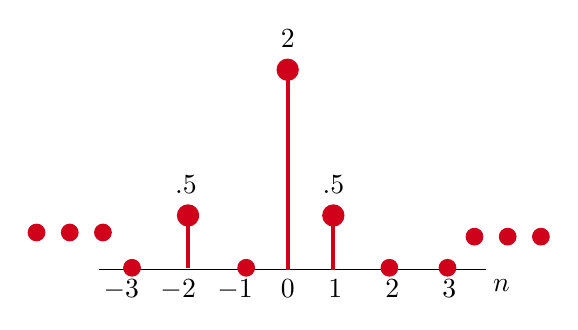
\begin{tikzpicture}[x=0.75pt,y=0.75pt,yscale=-1,xscale=1]
%uncomment if require: \path (0,437); %set diagram left start at 0, and has height of 437

%Straight Lines [id:da6960321259995674] 
\draw    (311.71,160) -- (125.29,160) ;
%Straight Lines [id:da40935280908685534] 
\draw [color={rgb, 255:red, 208; green, 2; blue, 27 }  ,draw opacity=1 ][line width=1.5]    (216,63.58) -- (216,160) ;
\draw [shift={(216,63.58)}, rotate = 90] [color={rgb, 255:red, 208; green, 2; blue, 27 }  ,draw opacity=1 ][fill={rgb, 255:red, 208; green, 2; blue, 27 }  ,fill opacity=1 ][line width=1.5]      (0, 0) circle [x radius= 4.36, y radius= 4.36]   ;
%Straight Lines [id:da27098747867922146] 
\draw [color={rgb, 255:red, 208; green, 2; blue, 27 }  ,draw opacity=1 ][line width=1.5]    (238,133.79) -- (238,160) ;
\draw [shift={(238,133.79)}, rotate = 90] [color={rgb, 255:red, 208; green, 2; blue, 27 }  ,draw opacity=1 ][fill={rgb, 255:red, 208; green, 2; blue, 27 }  ,fill opacity=1 ][line width=1.5]      (0, 0) circle [x radius= 4.36, y radius= 4.36]   ;
%Straight Lines [id:da13999635812051947] 
\draw [color={rgb, 255:red, 208; green, 2; blue, 27 }  ,draw opacity=1 ][line width=1.5]    (168,133.79) -- (168,159) ;
\draw [shift={(168,133.79)}, rotate = 90] [color={rgb, 255:red, 208; green, 2; blue, 27 }  ,draw opacity=1 ][fill={rgb, 255:red, 208; green, 2; blue, 27 }  ,fill opacity=1 ][line width=1.5]      (0, 0) circle [x radius= 4.36, y radius= 4.36]   ;
%Shape: Circle [id:dp7665960437062732] 
\draw  [color={rgb, 255:red, 208; green, 2; blue, 27 }  ,draw opacity=1 ][fill={rgb, 255:red, 208; green, 2; blue, 27 }  ,fill opacity=1 ] (137,159) .. controls (137,156.79) and (138.79,155) .. (141,155) .. controls (143.21,155) and (145,156.79) .. (145,159) .. controls (145,161.21) and (143.21,163) .. (141,163) .. controls (138.79,163) and (137,161.21) .. (137,159) -- cycle ;
%Shape: Circle [id:dp436359616871549] 
\draw  [color={rgb, 255:red, 208; green, 2; blue, 27 }  ,draw opacity=1 ][fill={rgb, 255:red, 208; green, 2; blue, 27 }  ,fill opacity=1 ] (192,159) .. controls (192,156.79) and (193.79,155) .. (196,155) .. controls (198.21,155) and (200,156.79) .. (200,159) .. controls (200,161.21) and (198.21,163) .. (196,163) .. controls (193.79,163) and (192,161.21) .. (192,159) -- cycle ;
%Shape: Circle [id:dp9890944921306494] 
\draw  [color={rgb, 255:red, 208; green, 2; blue, 27 }  ,draw opacity=1 ][fill={rgb, 255:red, 208; green, 2; blue, 27 }  ,fill opacity=1 ] (261,159) .. controls (261,156.79) and (262.79,155) .. (265,155) .. controls (267.21,155) and (269,156.79) .. (269,159) .. controls (269,161.21) and (267.21,163) .. (265,163) .. controls (262.79,163) and (261,161.21) .. (261,159) -- cycle ;
%Shape: Circle [id:dp881688459697376] 
\draw  [color={rgb, 255:red, 208; green, 2; blue, 27 }  ,draw opacity=1 ][fill={rgb, 255:red, 208; green, 2; blue, 27 }  ,fill opacity=1 ] (289,159) .. controls (289,156.79) and (290.79,155) .. (293,155) .. controls (295.21,155) and (297,156.79) .. (297,159) .. controls (297,161.21) and (295.21,163) .. (293,163) .. controls (290.79,163) and (289,161.21) .. (289,159) -- cycle ;
%Shape: Circle [id:dp9509429138475404] 
\draw  [color={rgb, 255:red, 208; green, 2; blue, 27 }  ,draw opacity=1 ][fill={rgb, 255:red, 208; green, 2; blue, 27 }  ,fill opacity=1 ] (123,142) .. controls (123,139.79) and (124.79,138) .. (127,138) .. controls (129.21,138) and (131,139.79) .. (131,142) .. controls (131,144.21) and (129.21,146) .. (127,146) .. controls (124.79,146) and (123,144.21) .. (123,142) -- cycle ;
%Shape: Circle [id:dp9940340579577291] 
\draw  [color={rgb, 255:red, 208; green, 2; blue, 27 }  ,draw opacity=1 ][fill={rgb, 255:red, 208; green, 2; blue, 27 }  ,fill opacity=1 ] (107,142) .. controls (107,139.79) and (108.79,138) .. (111,138) .. controls (113.21,138) and (115,139.79) .. (115,142) .. controls (115,144.21) and (113.21,146) .. (111,146) .. controls (108.79,146) and (107,144.21) .. (107,142) -- cycle ;
%Shape: Circle [id:dp3557855538501913] 
\draw  [color={rgb, 255:red, 208; green, 2; blue, 27 }  ,draw opacity=1 ][fill={rgb, 255:red, 208; green, 2; blue, 27 }  ,fill opacity=1 ] (91,142) .. controls (91,139.79) and (92.79,138) .. (95,138) .. controls (97.21,138) and (99,139.79) .. (99,142) .. controls (99,144.21) and (97.21,146) .. (95,146) .. controls (92.79,146) and (91,144.21) .. (91,142) -- cycle ;
%Shape: Circle [id:dp49757143963020933] 
\draw  [color={rgb, 255:red, 208; green, 2; blue, 27 }  ,draw opacity=1 ][fill={rgb, 255:red, 208; green, 2; blue, 27 }  ,fill opacity=1 ] (334,144) .. controls (334,141.79) and (335.79,140) .. (338,140) .. controls (340.21,140) and (342,141.79) .. (342,144) .. controls (342,146.21) and (340.21,148) .. (338,148) .. controls (335.79,148) and (334,146.21) .. (334,144) -- cycle ;
%Shape: Circle [id:dp1192153550884405] 
\draw  [color={rgb, 255:red, 208; green, 2; blue, 27 }  ,draw opacity=1 ][fill={rgb, 255:red, 208; green, 2; blue, 27 }  ,fill opacity=1 ] (318,144) .. controls (318,141.79) and (319.79,140) .. (322,140) .. controls (324.21,140) and (326,141.79) .. (326,144) .. controls (326,146.21) and (324.21,148) .. (322,148) .. controls (319.79,148) and (318,146.21) .. (318,144) -- cycle ;
%Shape: Circle [id:dp8865578210167575] 
\draw  [color={rgb, 255:red, 208; green, 2; blue, 27 }  ,draw opacity=1 ][fill={rgb, 255:red, 208; green, 2; blue, 27 }  ,fill opacity=1 ] (302,144) .. controls (302,141.79) and (303.79,140) .. (306,140) .. controls (308.21,140) and (310,141.79) .. (310,144) .. controls (310,146.21) and (308.21,148) .. (306,148) .. controls (303.79,148) and (302,146.21) .. (302,144) -- cycle ;

% Text Node
\draw (313.71,163.4) node [anchor=north west][inner sep=0.75pt]    {$n$};
% Text Node
\draw (216,163.4) node [anchor=north] [inner sep=0.75pt]    {$0$};
% Text Node
\draw (190.66,163.4) node [anchor=north] [inner sep=0.75pt]    {$-1$};
% Text Node
\draw (163.24,163.4) node [anchor=north] [inner sep=0.75pt]    {$-2$};
% Text Node
\draw (135.82,163.4) node [anchor=north] [inner sep=0.75pt]    {$-3$};
% Text Node
\draw (239,163.4) node [anchor=north] [inner sep=0.75pt]    {$1$};
% Text Node
\draw (266.42,163.4) node [anchor=north] [inner sep=0.75pt]    {$2$};
% Text Node
\draw (293.84,163.4) node [anchor=north] [inner sep=0.75pt]    {$3$};
% Text Node
\draw (167,124.39) node [anchor=south] [inner sep=0.75pt]    {$.5$};
% Text Node
\draw (238,124.39) node [anchor=south] [inner sep=0.75pt]    {$.5$};
% Text Node
\draw (216,54.18) node [anchor=south] [inner sep=0.75pt]    {$2$};


\end{tikzpicture}

          \caption{Even $x[n]$}
          \label{fig:20}
        \end{figure}

        and then the odd:

        \begin{figure}[H]
          \centering
          \include{Figures/Fig6-2}
          \caption{Odd $x[-n]$}
          \label{fig:21}
        \end{figure}

  \item Express the real part of each of the following signals in the form $Ae^{-at}\cos(\omega t + \phi)$ where $A$, $a$, $\omega$ and $\phi$ are real numbers with $A > 0$ and $-\pi < \phi \leq \pi$.

    \begin{enumerate}

      \item $x_1(t)=4e^{-2t}\sin\left( 10t+\frac{3\pi}{4}\right)\cos\left( 10t+\frac{3\pi}{4} \right)$

        \begin{center}
          Per trig identities, we can rewrite this as:
        \end{center}
        $$2e^{-2t}\sin\left( 20t+\frac{3\pi}{2}\right) \right)$$
        \begin{center}
          Per another identity, we can convert $\sin\to\cos$:
        \end{center}
        $$2e^{-2t}\cos\left( \frac{\pi}{2}-20t-\frac{3\pi}{2}\right) \right)$$
        $$x_1(t)=2e^{-2t}\cos\left( -20t-\pi\right) \right)$$
        \begin{center}
          Since $\cos(x)=\cos(-x)$, we finally write:
        \end{center}
        $$\boxed{x_1(t)=2e^{-2t}\cos\left( 20t+\pi\right) \right)}$$

      \item $x_2(t)=j(1-j)e^{(-5+j\pi)t}$

        We can rewrite this in terms of exponentials:

        $$x_2(t)=e^{\frac{\pi}{2}j}\left( \sqrt{2}e^{-\frac{\pi}{4}j} \right)\left( e^{(-5+j\pi)t} \right)$$
        $$x_2(t)=\sqrt{2}e^{-5t}\left( e^{j\pi t+\frac{\pi}{2}j-\frac{\pi}{4}j} \right)$$
        $$x_2(t)=\sqrt{2}e^{-5t}\left( e^{j(\pi t+\frac{\pi}{4})} \right)$$
        $$\boxed{x_2(t)=\sqrt{2}e^{-5t}\cos\left(\pi t+\frac{\pi}{4}\right)}$$

    \end{enumerate}

  \item Determine whether each of the following continuous time signals is periodic. If the signal is periodic, determine its fundamental period.

    \begin{enumerate}

      \item $x(t)=5\cos\left( 400\pi t+\frac{\pi}{4} \right)$

        The function is periodic, with angular frequency $\omega=400\pi\left[ \dfrac{\text{rad}}{\si{\second}} \right]$

        This gives us the fundamental period:

        $$\boxed{T=\frac{2\pi}{400\pi}=.005[\si{\second}]}$$

      \item $x(t)=20e^{j(\pi t-2)}$

        The function is periodic, with angular frequency $\omega=\pi\left[ \dfrac{\text{rad}}{\si{\second}} \right]$

        This gives us the fundamental period:

        $$\boxed{T=\frac{2\pi}{\pi}=2[\si{\second}]}$$

      \item $x(t)=2\left[ \sin\left( 50\pi t - \frac{\pi}{3} \right) \right]^2$

        The function is periodic, with angular frequency $\omega=50\pi\left[ \dfrac{\text{rad}}{\si{\second}} \right]$

        This gives us the fundamental period:

        $$\boxed{T=\frac{2\pi}{50\pi}=.04[\si{\second}]}$$

      \item $x(t)=\left\{\begin{array}{l r} 2\sin(5\pi t),\, & t\geq 0\\ -2\sin(-5\pi t),\, &t<0\end{array}$

        Per trigonometric identities, we know that:

        $$\sin(t)=-\sin(-t)$$

        Thus, the function presented is simply:

        $$x(t)=2\sin(5\pi t)$$

        This function is periodic, with angular frequency $\omega=5\pi\left[ \dfrac{\text{rad}}{\si{\second}} \right]$

        This gives us the fundamental period:

        $$\boxed{T=\frac{2\pi}{5\pi}=.4[\si{\second}]}$$

    \end{enumerate}

  \item Determine whether each of the following discrete time signals is periodic. If the signal is periodic, determine its fundamental period.

    \begin{enumerate}

      \item $x[n]=2\cos\left( \frac{7}{11}n+\frac{\pi}{2} \right)$

        To be periodic, $(2\pi/\Omega_o)m$ must be rational. We see:

        $$\Omega_o=\frac{7}{11}\to\frac{22\pi m}{7}$$

        As a result of the $\pi$, this is never rational and therefore not periodic.

      \item $x[n]=\cos(\pi n)+4\sin\left( \frac{\pi}{4}n^2 \right)$

        To be periodic, both sinusoids must have $2\pi/\Omega_o$ be rational. We see:

        $$\Omega_1=\pi\to\frac{2\pi}{\pi}=2\text{ and }\Omega_2=\pi/4\to\frac{2\pi}{\pi/4}=8$$

        Thus, the function is periodic. The period is the smallest number such that the two periods are a common divisor of the integer. Since 8 is divisible by 2, \underline{the fundamental period is 8}.

      \item $x[n]=3\sin\left( \frac{\pi}{3}n \right)+\cos\left( \frac{\pi}{4}n \right)-3\cos\left( \frac{\pi}{6}n+\frac{\pi}{3} \right)$ 

        Once again, each of the sinusoids must be periodic:

        $$\Omega_1=\pi/3\to\frac{2\pi}{\pi/3}=6\text{ and }\Omega_2=\pi/4\to\frac{2\pi}{\pi/4}=8\text{ and }\Omega_3=\pi/6\to\frac{2\pi}{\pi/6}=12$$

        Thus, we see these functions are all periodic. The smallest integer which is divisible by all of these values is 24, and, thus, \underline{the fundamental period is 24}.

    \end{enumerate}

\end{enumerate}

\end{document}

